\documentclass[13pt,a4paper]{extreport}
\usepackage[utf8]{inputenc}
\usepackage[utf8]{vietnam}
\usepackage{amsmath}
\usepackage{amsfonts}
\usepackage{amssymb}
\usepackage{graphicx}
\usepackage{color}
\graphicspath{ {images/} }
\usepackage{enumerate}
\usepackage{multirow}
\usepackage{listings}
\usepackage{indentfirst}
\usepackage[unicode]{hyperref}
%\usepackage[unicode, hidelinks=true]{hyperref} %Tu dong tao bookmark
%\hypersetup{colorlinks = true}
\usepackage[left=2.5cm,right=2cm,top=2cm,bottom=2cm]{geometry}
%\usepackage[toc,page]{appendix}
\definecolor{dkgreen}{rgb}{0,0.6,0}
\definecolor{gray}{rgb}{0.5,0.5,0.5}
\definecolor{mauve}{rgb}{0.58,0,0.82}

\lstset{frame=tb,
  language=C,
  aboveskip=3mm,
  belowskip=3mm,
  showstringspaces=false,
  columns=flexible,
  basicstyle={\small\ttfamily},
  numbers=left,
  numberstyle=\tiny\color{gray},
  keywordstyle=\color{blue},
  commentstyle=\color{dkgreen},
  stringstyle=\color{mauve},
  breaklines=true,
  captionpos=t,
  breakatwhitespace=true,
  tabsize=2
}
\begin{document}

\begin{titlepage}
	\centering
	\begin{small}
\bfseries{TRƯỜNG ĐẠI HỌC KỸ THUẬT -- CÔNG NGHỆ CẦN THƠ\\KHOA ĐIỆN TỬ -- VIỄN THÔNG\\ \vspace{1cm}}
   \end{small}
	
\includegraphics[width=.3\textwidth]{CTUT_logo}\par\vspace{1cm}
	{\Large\bfseries ĐỒ ÁN MÔN HỌC VI ĐIỀU KHIỂN\vspace{.5cm}\par}
	{\Large\bfseries ĐỀ TÀI\vspace{.5cm}\par}
	{\Large\bfseries ĐỌC GIÁ TRỊ NHIỆT ĐỘ ĐIỀU KHIỂN\\ BƠM NƯỚC CỨU HỎA\par}
	\vspace{2cm}
	
	\begin{tabular}{ll}
	{\Large\itshape Giảng viên hướng dẫn:} & {\Large\itshape Thầy Đường Khánh Sơn}\vspace{.3cm}\\
	{\Large\itshape Nhóm sinh viên thực hiện:} &{\Large\itshape Nhóm 7}\vspace{.2cm}\\
		{\Large\itshape \hspace{1.5cm}1. Nguyễn Văn Đình}& {\Large\itshape -- MSSV: 1350353}\vspace{.2cm}\\
	{\Large\itshape \hspace{1.5cm}2. Thi Minh Nhựt}& {\Large\itshape -- MSSV: 1350366}\vspace{.2cm}\\
	{\Large\itshape \hspace{1.5cm}3. Phạm Thanh Quý}& {\Large\itshape -- MSSV: 1350222}\vspace{.2cm}\\
		{\Large\itshape \hspace{1.5cm}4. Liên Thái Trường}& {\Large\itshape -- MSSV: 1350358}\vspace{.2cm}\\
		{\Large\itshape \hspace{1.5cm}5. Lư Anh Tuấn}& {\Large\itshape -- MSSV: 1350240}\vspace{.2cm}\\
	\end{tabular}
	
	\vfill
	
	
	\vfill
	
% Bottom of the page
	{\large \textit{Cần Thơ\\ \today}\par}
\end{titlepage}
\pagenumbering{roman}
\tableofcontents
 
\thispagestyle{empty}
 
\listoffigures
 
\listoftables
 
\newpage
 
\pagenumbering{arabic}

\part*{NỘI DUNG BÁO CÁO}
\addcontentsline{toc}{part}{NỘI DUNG BÁO CÁO}
\chapter*{Giới thiệu về đề tài}
\addcontentsline{toc}{chapter}{Giới thiệu về đề tài}
%\chapter*{Giới thiệu về đề tài}
Em chân thành cảm ơn thầy Đường Khánh Sơn đã nhận xét và góp ý cho nhóm em để hoàn thiện bài báo cáo hơn. Em xin tiếp nhận ý kiến và sẽ bổ sung, hoàn thiện thêm một số tín năng nữa: thu thập số liệu, cải tiến lại việc bơm nước (tính đến thời gian động cơ bơm nước lên). Chân thành cảm ơn thầy!
\begin{itemize}
\item \textbf{\textit{Tên đề tài}}: Đọc giá trị nhiệt độ điều khiển bơm nước cứu hỏa.
\item \textbf{\textit{Nội dung đề tài}}: Sử dụng \emph{vi điều khiển PIC 16F887} đọc giá trị nhiệt độ từ \emph{cảm biến nhiệt độ DS18B20} để \emph{điều khiển việc tưới nước tự động} thông qua việc \emph{kích Relay} để \emph{đóng, mở} khởi động động cơ bơm nước. Đề tài sử dụng động cơ DC để mô phỏng cho chương trình.
\end{itemize}

Dù nhóm em đã cố gắng hoàn thành thật tốt, nhưng không tránh khỏi thiếu sót, mong thầy và các bạn nhận xét, cho ý kiến để bài báo cáo của nhóm được hoàn thiện hơn.
\begin{flushright}
\textit{Nhóm sinh viên thực hiện}\vspace{.5cm}\\
Nhóm 7
\end{flushright}
\chapter{Phần cứng}
\section{Danh sách phần cứng}
\begin{table}[!h]
\begin{center}
\begin{tabular}{|c|p{6cm}|p{7.5cm}|l}\cline{1-3}
\textbf{STT} & \centering{\textbf{Phần cứng}} & \centering{\textbf{Mô tả}} & \\ \cline{1-3}
1 & PIC 16F887 & Vi điều khiển & \\ \cline{1-3}
2 & Mạch nạp PICKit2 K150 & Nạp chương trình cho PIC & \\ \cline{1-3}
3 & Cảm biến DS18B20 (loại dây) & Đo nhiệt độ  & \\ \cline{1-3}
4 & LCD 1602 & Màn hình hiển thị   & \\ \cline{1-3}
5 & Relay với Opto cách ly & Đóng mở motor & \\ \cline{1-3}
6 & Động cơ 5VDC & Dùng để bơm nước (chạy demo)  & \\ \cline{1-3}
7 & Nguồn 5VDC - 2A & Cấp nguồn cho vi điều khiển & \\ \cline{1-3}
8 & Nút nhấn 4 chân: 13 nút & Làm bàn phím và nút Reset  & \\ \cline{1-3}
9 & Điện trở $4.7k\Omega$: 14 điện trở & Tạo điện trở Pullup  & \\ \cline{1-3}
10 & Biến trở $10k\Omega$ & Chỉnh độ tương phản của LCD  & \\ \cline{1-3}
11 & Thạch anh $20MHz$ & Làm mạch dao động cho vi điều khiển  & \\ \cline{1-3}
12 & Tụ điện $15pF$: 2 tụ & Kết hợp tạo mạch dao động. & \\ \cline{1-3}
13 & Domino 3 chân & Đấu nối dây cho cảm biến nhiệt độ  & \\ \cline{1-3}
14 & Đế IC 40 chân & Để gắn vi điều khiển PIC 16F887 lên  & \\ \cline{1-3}
15 & Rào cái loại đơn & Ra chân cho LCD  & \\ \cline{1-3}
16 & Rào đực loại đơn: 2 rào & Ra chân cua PIC 16F887  & \\ \cline{1-3}
17 & Dây kết nối 2 đầu cái cái & Dùng để kết nối các chân với nhau  & \\ \cline{1-3}
18 & Test board hàn mạch: 2 cái & Hàn linh kiện lên đây  & \\ \cline{1-3}
19 & Các dụng cụ khác, \ldots &  & \\ \cline{1-3}
\end{tabular}
\end{center}
\caption{Mô tả phần cứng dùng được dùng cho đề tài}
\end{table}
Trong \textit{phụ lục \ref{phancung-sodo}} em có trình bày hình ảnh của các linh kiện trên trong thực tế.
\newpage
\section{Vi điều khiển PIC 16F887}
\subsection{Sơ đồ chân}
\begin{figure}[!h]
\begin{center}
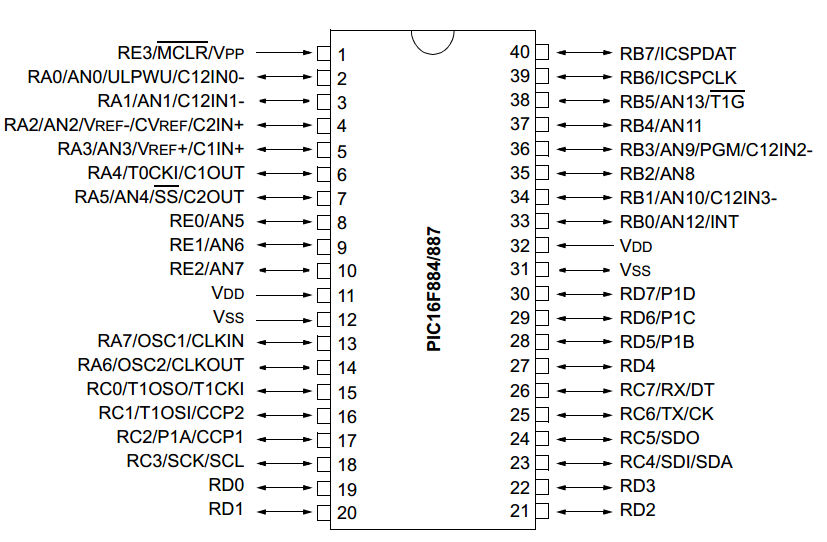
\includegraphics[scale=.8]{PIC16F887}
\end{center}
\caption{Sơ đồ chân của PIC 16F887}
\end{figure}
\subsection{Làm mạch điều khiển}
\begin{enumerate}[{\bf a.}]
\item \textbf{Các thành phần cơ bản:} \textit{cấp nguồn, mạch dao động, mạch reset, xếp thứ tự các chân}
\begin{itemize}
\item \textit{Cấp nguồn cho vi điều khiển}: sử dụng nguồn DC -- 5V.\\
\begin{table}[h]
\begin{center}
\begin{tabular}{|c|p{5cm}|l} \cline{1-2}
\textbf{Nguồn DC -- 5V} & \centering{\textbf{PIC 16F887}} &\\ \cline{1-2}
5V & \textit{Chân VDD}: số 11 và số 32 &\\ \cline{1-2}
0V & \textit{Chân VSS}: số 12 và số 31 &\\ \cline{1-2}
\end{tabular}
\end{center}
\caption{Cách cấp nguồn cho vi điều khiển PIC 16F887} \label{capnguon}
\end{table}
$\ast$\textit{Lưu ý}: Sử dụng cả 4 chân: số $11,12,31,32$.
\item \textit{Làm mạch dao động cho vi điểu khiển}: lựa cho giá trị tụ điện và tần số thạch anh thích hợp.
\begin{itemize}
\item \emph{Thạch anh:} Để thực hiện các lệnh trong vi điều khiển, cần phải tạo ra xung nhịp, tần số xung nhịp phụ thuộc vào thạch anh gắn vào vi điều khiển. Nhiệm vụ chính của thạch anh là tạo ra dao động ổn định.
\item \emph{Tụ điện}: sử dụng hai tụ điện mắc vào để tăng tính ổn định tần số (tụ bù nhiệt ổn tầng).
\item Sử dụng mạch tạo dao động với thạch anh ổn định hơn mạch dao động $RC$.
\item Cách kiểm tra thạch anh: Sử dụng \emph{VOM} ở giai \emph{đo tần số}, đo hai đầu của thạch anh, nếu \emph{tần số bằng tần số ghi trên thạch anh} thì \emph{thạch anh còn tốt}, còn ngược lại thì thạch anh bị hỏng.
\begin{table}[h]
\begin{center}
\begin{tabular}{|c|l|} \hline
\textbf{Thạch anh} & \textbf{PIC 16F887}\\ \hline
2 chân & \textit{Chân OSC1/CLKI và OSC2/CLKO}:\\
$20MHz$ và 2 tụ $15pF$ &  chân số 13 và số 14\\ \hline
\end{tabular}
\end{center}
\caption{Cách mắc thạch anh cho vi điều khiển PIC 16F887}
\end{table}
\item[$\ast$] \textit{Trong mạch thiết kế của đề tài: sử dụng thạch anh $20MHz$ và hai tụ điện có giá trị $15pF$ để tạo mạch dao động cho vi điều khiển.}
\end{itemize}
\item \textit{Tạo mạch Reset cho vi điều khiển:} sử dụng chân $MCLR/V_{PP}$. Bình thường chân này ở mức $1$ (mức cao), để reset vi điều khiển, đưa chân $MCLR/V_{PP}$ xuống mức $0$ (mức thấp). Xem hình \ref{fmachdaodongreset}
\item \textit{Sơ đồ nguyên lý}: được vẽ bằng phần mềm \emph{Protues}.
%\item[$\circledast$] \textit{Sơ đồ kết nối thực tế}: được vẽ bằng phần \emph{Fritzing} \footnote{http://fritzing.org/home/}
\begin{figure}[h]
\begin{center}
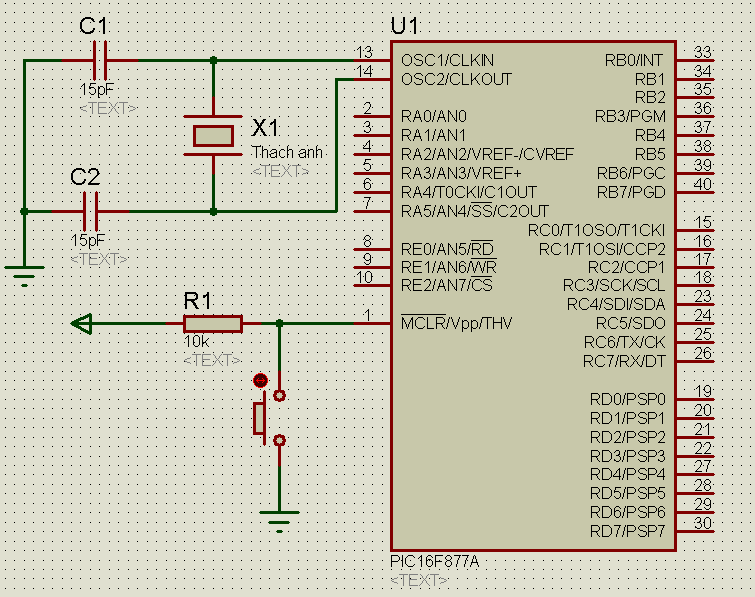
\includegraphics[scale=.5]{MachDaoDong-Reset}
\end{center}
\caption{Cách mắc mạch dao động bằng thạnh anh cho PIC 16F877A} \label{fmachdaodongreset}
\end{figure}
\item \textit{Có thể tạo thêm LED báo nguồn và LED báo Reset cho vi điều khiển để cho mạch có tính rõ ràng}.
\end{itemize}
\item \textbf{Kiểm tra mạch đã hàn}: Sau khi hàn mạch xong, sử dụng VOM \textit{kiểm tra xem có ngắn mạch} giữa các chân với nhau không, phải đảm bảo là không có ngắn mạch giữa các chân thì mới sử dụng mạch thiết kế, nếu không sẽ gây hỏng PIC 16F887 hoặc mạch chạy không theo đúng chức năng đã lập trình.
\end{enumerate}
\section{Màn hình hiển thị LCD}
\subsection{Sơ đồ chân và chức năng của các chân trong LCD}
\hspace{.6cm}\textit{Module LCD} (xem hình \ref{LCD1602} trong phụ lục \ref{phuluc-phancung}): có $16$ chân kết nối được đánh số theo thứ tự $1 - 16$ và được ghi trên LCD. Ta sẽ tìm hiểu chức năng của các chân này:
\begin{table}[h]
\begin{center}
\begin{tabular}{|c|c|p{6.5cm}|p{5cm}|l}\cline{1-4}
\textbf{STT} & \textbf{Ký hiệu} & \centering{\textbf{Mô tả}} & \centering{\textbf{Giá trị}} &\\ \cline{1-4}
1 & VSS & GND & $0V$ &\\ \cline{1-4}
2 & VCC & & $5V$ &\\ \cline{1-4}
3 & VEE & Tùy chỉnh độ tương phản & &\\ \cline{1-4}
\multirow{2}{.5cm}{ 4} & \multirow{2}{.8cm}{RS} & \multirow{2}{5cm}{Lựa chọn thanh ghi} & RS = 0: ghi lệnh & \\
& & & RS = 1: ghi dữ liệu &\\ \cline{1-4}
\multirow{2}{.5cm}{ 5} & \multirow{2}{.8cm}{R/W} & \multirow{2}{7cm}{Chọn thanh ghi đọc/viết dữ liệu} & R/W = 0: viết dữ liệu & \\
& & & R/W = 1: đọc dữ liệu &\\ \cline{1-4}
6 & E & Enable & &\\ \cline{1-4}
7 & DB0 & \multirow{8}{5cm}{Chân chuyền dữ liệu} & \multirow{8}{5cm}{8 bit từ $DB0 \rightarrow DB7$} & \\ 
8 & DB1 &  & & \\ 
9 & DB2 &  & & \\ 
10 & DB3 &  & & \\ 
11 & DB4 &  & & \\ 
12 & DB5 &  & & \\ 
13 & DB6 &  & & \\ 
14 & DB7 &  & &\\ \cline{1-4}
15 & A & Cực dương của LED nền & $0 - 5V$&\\ \cline{1-4}
16 & K & Cực âm của LED nền & $0V$ &\\ \cline{1-4}
\end{tabular}
\end{center}
\caption{Sơ đồ chân và chứa năng các chân trong LCD} \label{cnLCD}
\end{table}
\subsection{Kết nối LCD với vi điều khiển PIC 16F887}
\begin{itemize}
\item Có 2 cách truyền dữ liệu: truyền cả 8 bit dữ liệu (từ $DB0 \rightarrow DB7$ hoặc truyền 4 bit dữ liệu (từ $DB4 \rightarrow DB7$). Chọn cách truyền \textit{4 bit dữ liệu}.
\item \textit{Cách kết nối}: xem bảng \ref{conLCD}.
\newpage
\begin{table}[!h]
\begin{center}
\begin{tabular}{|l|c|c|}\hline
\textbf{LCD 16x2} & \textbf{PIC 16F887} & \\ \hline
VSS: \textit{số 1} & VSS: \textit{số 12} & \\ \hline
VCC: \textit{số 2} & VDD: \textit{số 11} & \\ \hline
VEE: \textit{số 3} & & Biến trở $10k\Omega$ \\ \hline
RS: \textit{số 4} & RD1: \textit{số 20} & \\ \hline
R/W: \textit{số 5} & RD2: \textit{số 21} & \\ \hline
E: số 6 & RD3: số 22 & \\ \hline
DB4: \textit{số 11} & RD4: \textit{số 23} & \\ \hline
DB5: \textit{số 12} & RD5: \textit{số 28} & \\ \hline
DB6: \textit{số 13} & RD6: \textit{số 29} & \\ \hline
DB7: \textit{số 14} & DB7: \textit{số 30} & \\ \hline
A: \textit{số 15} & VDD: \textit{số 11} & \\ \hline
K: \textit{số 16} & VSS: \textit{số 12} & \\ \hline
\end{tabular}
\end{center}
\caption{Cách kết nối LCD với vi điều khiển PIC 16F887} \label{conLCD}
\end{table}
\item \textit{Sơ đồ nguyên lý}: vẽ bằng phần mềm Protues.
\begin{figure}[h]
\begin{center}
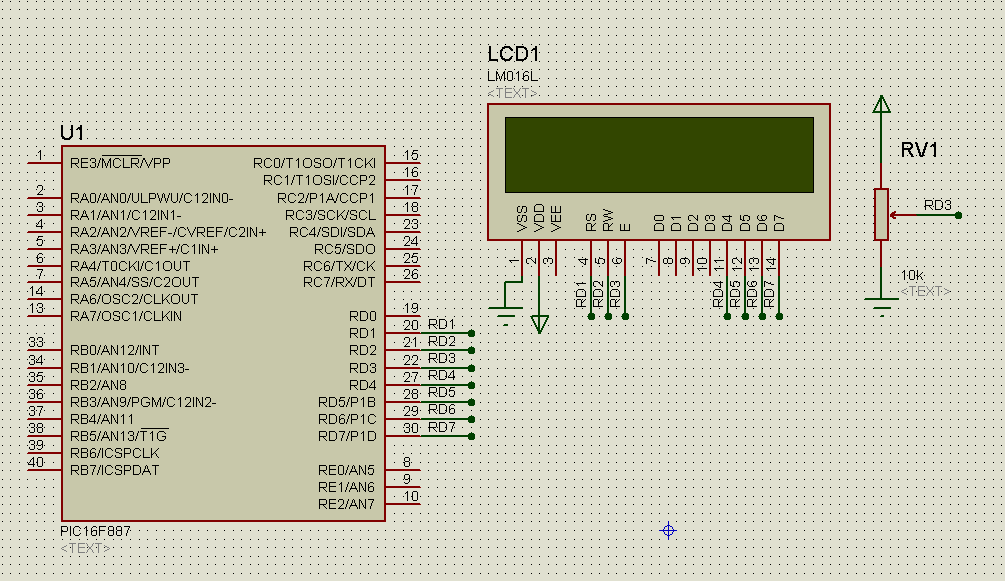
\includegraphics[scale=.5]{MachLCD}
\end{center}
\caption{Cách kết nối LCD với vi điều khiển PIC 16F887}
\end{figure}
\end{itemize}
\subsection{Tập lệnh của LCD}
\hspace{.6cm}Chúng ta có thể tìm hiểu các hướng dẫn trên các trang Internet hoặc trong tài liệu tham khảo \verb|Systronix_20x4_lcd_brief_data.pdf| để hiểu rõ các lệnh của LCD.
\subsection{Điều khiển LCD}
\begin{itemize}
\item Ta quan tâm đến việc hiển thị lên LCD. Tức ghi giá trị và cho hiển thị lên LCD. Dùng lệnh: \verb|Output_low(LCD_RW);| $\longrightarrow$ đưa chân \verb|R/W = 0| để thực hiện chế độ ghi (xem bảng \ref{cnLCD}) và các chân được định nghĩa trong file \verb|DEF_PIN.H| (xem mục \ref{defpin} của phụ lục \ref{lib}).
\item Sử dụng các hàm được định nghĩa trong file \verb|LCD_LIB_4BIT.C| của mục \ref{libLCD} trong phụ lục \ref{lib}:
\begin{itemize}
\item Hiển thị ký tự, chuỗi hoặc số lên LCD: dùng \verb|LCD_PutChar(unsigned int cX);|
\begin{itemize}
\item Ký tự hoặc chuỗi: \textit{ví dụ}: hiển thị chuỗi \verb|"HELLO LCD"| thì ta dùng dòng lệnh sau:
\begin{verbatim}
printf(LCD_PutChar,"HELLO LCD");
\end{verbatim}
\item Số: số thực hoặc số nguyên, thì ta định dạng: \verb|%d| (số nguyên) hoặc \verb|%lu| (với số nguyên dài) hoặc \verb|%f| (với số thực), \textit{ví dụ}: hiện thị số \verb|123| hoặc \verb|1.23| thì ta dùng lệnh sau:
\begin{verbatim}
printf(LCD_PutChar,"%d",123); //Hiển thị số nguyên

//Hiển thị số thực với 2 chữ số thập phân sau dấu phẩy
printf(LCD_PutChar,"%.2f",1.23); 
\end{verbatim}
\end{itemize}
\item Vị trí con trỏ: dùng hàm \verb|LCD_SetPosition(unsigned int cX);|
\begin{itemize}
\item Chuyển đến vị trí đầu tiên của dòng 1: \verb|LCD_SetPosition(0x00);|, tăng giá trị lên để chuyển đến những vị trí tiếp theo dòng 1.
\item Chuyển đến vị trí đầu tiên của dòng 2: \verb|LCD_SetPosition(0x40;)|, tăng giá trị lên để chuyển đến những vị trí tiếp theo dòng 2.
\end{itemize}
\item Xóa màn hình: dùng lệnh \verb|LCD_PutCmd(0x01);|
\item[$\ast$] Các lệnh trên là các lệnh được sử dụng để thao tác với LCD trong phạm vi đề tài.
\end{itemize}
\item Để sử dụng được thư viện \verb|LCD_LIB_4BIT.C| cần chép chung các file \verb|DEF_887.H;| \verb| DEF_PIN.H;| \verb|LCD_LIB_4BIT.C| và một số khai báo cơ bản khi viết chương trình bằng ngôn ngữ CCS.
\end{itemize}
\section{Cảm biến nhiệt độ DS18B20}
\subsection{Thông số kỹ thuật}
\begin{itemize}
\item Là IC cảm biến nhiệt độ có 3 chân: VCC, GND và DATA.
\item Giao tiếp thông qua \textit{giao thức một dây} với vi xử lý.
\item Đặc điểm chính:
\begin{itemize}
\item Cung cấp nhiệt độ với độ phân giải $12bit$.
\item Khoảng nhiệt độ rộng: $-10 \div 125^0C$.
\item Sai số cho phép: $\pm0.5^0C$.
\item Có chức năng cảnh báo nhiệt khi nhiệt độ vượt ngưỡng cho phép. Bộ nhớ nhiệt độ cảnh báo không bị mất khi mất nguồn.
\item Có mã nhận diện lên đến 64-bit, vì vậy ta có thể kiểm tra nhiệt độ với nhiều IC DS18B20 mà chỉ dùng 1 dây dẫn duy nhất để giao tiếp với các IC này.
\end{itemize}
\item Để biết nhiều thông số hơn, ta có thể xem trong Datasheet của IC với tên là \verb|DS18B20.pdf|.
\end{itemize}
\subsection{Sơ đồ chân và các kết nối với vi điều khiển PIC16F887}
\begin{itemize}
\item IC DS18B20 có 3 chân: VCC, GND và DATA. Khi được tích hợp thành dây đo nhiệt độ (xem trong hình \ref{DS18B200} trong phần phụ lục \ref{phuluc-phancung}): \textit{Dây màu đỏ} -- VCC; \textit{Dây màu đen} -- GND; \textit{Dây màu vàng} hoặc \textit{Dây màu trắng} -- DATA.
\item Cách kết nối:
\begin{table}[h]
\begin{center}
\begin{tabular}{|p{7cm}|c|}\hline
\centering{\textbf{DS18B20}} & \textbf{PIC16F887} \\ \hline
Dây đỏ -- VCC & VDD \\ \hline
Dây đen -- GND & VSS \\ \hline
Dây vàng hoặc dây trắng -- DATA & RC1 \\ \hline
\multicolumn{2}{|c|}{Nối điện trở $4.7k\Omega$ giữa chân VCC và chân DATA}\\ 
\multicolumn{2}{|l|}{Để bit dữ liệu được kéo lên nguồn}\\ \hline
\end{tabular}
\end{center}
\caption{Kết nối DS18B20 với PIC16F887}
\end{table}
\item \textit{Sơ đồ nguyên lý}: vẽ bằng phần mềm Protues.
\begin{figure}[h]
\begin{center}
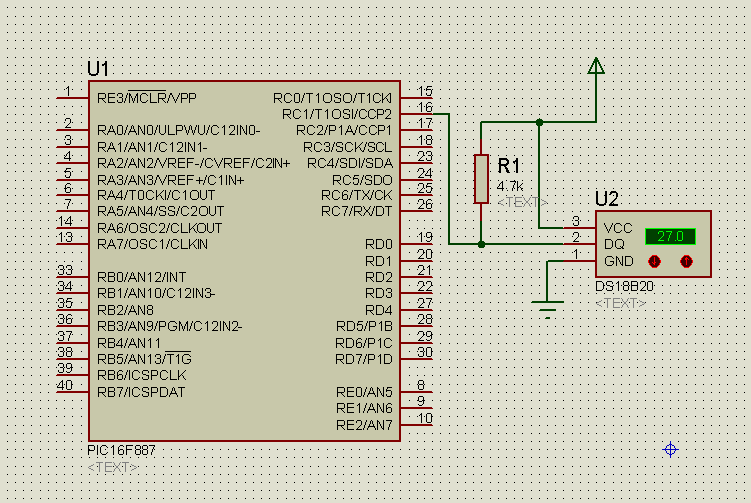
\includegraphics[scale=.5]{MachDS18B20}
\end{center}
\caption{Cách kết nối cảm biến nhiệt độ DS18B20 với vi điều khiển PIC16F887}
\end{figure}
\end{itemize}
\subsection{Giao thức giao tiếp một dây}
\begin{itemize}
\item \textit{Chuẩn giao tiếp một dây} -- $1 ~ WIRE$: là đường dẫn tín hiệu và đường dẫn điện áp nguồn nuôi có thể dùng chung trên một dây dẫn, nhiều cảm biến có thể dùng chung trên một đường dẫn (rất thích hợp với các ứng dụng đo lường đa điểm).
\item Các thiết bị \textit{Slave} kết nối \textit{cùng một bus} được phân biệt bởi \textit{64 bit địa chỉ}: Bắt đầu từ LBS:
\begin{itemize}
\item Byte đầu: mã của họ thiết bị có độ lớn 8 bit \textit{(8-bit family codes)}.
\item 6 byte tiếp theo: địa chỉ riêng của thiết bị.
\item Byte cuối: kiểm tra tính toàn vẹn của dữ liệu \textit{cyclic redundancy check -- CRC} có giá trị ứng với 7 byte đầu tiên.
\end{itemize}
\item Cách thức hoạt động:
\begin{itemize}
\item Bốn thao tác chính là: \textit{reset}, \textit{gửi bit 1}, \textit{gửi bit 0} và \textit{đọc bit}.
\item Mô tả 4 thao tác trên:
\begin{table}[h]
\begin{center}
\begin{tabular}{|l|p{4cm}|p{5cm}|l}\cline{1-3}
\textbf{Hoạt động} & \centering{\textbf{Mô tả}} & \centering{\textbf{Thực thi}} & \\ \cline{1-3}
Gửi bit 1 & Gửi bit 1 đến thiết bị Slave & Kéo bus xuống mưc thấp: $6\mu s$, nhả ra: $64 \mu s$ & \\ \cline{1-3}
Gửi bit 0 & Gửi bit 1 đến thiết bị Slave & Kéo bus xuống mưc thấp: $60\mu s$, nhả ra: $10 \mu s$ & \\ \cline{1-3}
Đọc bit & Đọc 1 bit & Kéo bus xuống mưc thấp: $6\mu s$, nhả ra: $9 \mu s$ $\longrightarrow$ đọc bit rồi delay $55\mu s$ & \\ \cline{1-3}
Reset & reset thiết bị Slave và chuẩn bị nhận lệnh & Kéo bus xuống mức thấp trong $480\mu s$ & \\ \cline{1-3}
\end{tabular}
\end{center}
\end{table}
\end{itemize}
\item File code \verb|ONEWIRE.C| của chuẩn giao tiếp một dây được trình bày trong mục \ref{ONEWIRE} của phụ lục \ref{lib}.
\end{itemize}
\subsection{Đọc nhiệt độ từ cảm biến DS18B20}
\begin{itemize}
\item Các lệnh ROM của DS18B200:
\begin{table}[!h]
\begin{center}
\begin{tabular}{|l|c|p{9cm}|l}\cline{1-3}
\centering{\textbf{Tên lệnh}} & \textbf{DATA} & \centering{\textbf{Chức năng}} & \\ \cline{1-3}
READ ROM & 33H & Đọc 64 bit ROM của DS18B20 \\ \hline
MATCH ROM & 33H & khi dùng nhiều DS18B20 thì cần phải dùng lệnh này xác nhận 64 bit ROM của một cảm biến& \\ \cline{1-3}
SKIP ROM & CCH & Truy cập đến bộ nhớ, bỏ qua xác nhận 64 bit ROM & \\ \cline{1-3}
SEARCH ROM & F0H & Tìm số DS18B20 được kết nối vào bus& \\ \cline{1-3}
ALARMSEARCH & ECH & Phản hồi khi nhiệt độ thấp hơn hoặc cao hơn ngưỡng cảnh báo đã cài đặt & \\ \cline{1-3}
\end{tabular}
\end{center}
\caption{Các lệnh trên ROM của DS18B20}
\end{table}
\newpage
\item Các lệnh thực thi của DS18B200:
\begin{table}[!h]
\begin{center}
\begin{tabular}{|l|c|p{9cm}|l}\cline{1-3}
\centering{\textbf{Tên lệnh}} & \textbf{DATA} & \centering{\textbf{Chức năng}} & \\ \cline{1-3}
WRITE SCRCHPAD & 4EH & Gửi 3 byte dữ liệu vào bộ nhớ nháp: Ngưỡng cảnh báo trên, ngưỡng cảnh báo dưới, cấu hình độ phâ giải cho phép đo & \\ \cline{1-3}
READ SCRCHPAD & BEH & Đọc nội dung của SCRCHPAD gồm 9 byte & \\ \cline{1-3}
COPY SCRCHPAD & 48H & Copy 2 byte, 3 byte, 4 byte từ SCRCHPAD vào ROM của DS18B20 & \\ \cline{1-3}
CONVERT T & 44H & Bắt đầu chuyển đổi nhiệt độ, kết quả lưu vào byte 0, byte 1 của SCRCHPAD. Thời gian chuyển đổi $\leq 200ms$& \\ \cline{1-3}
READ POWERSUPPLY & B4H & Một lệnh đọc sau lệnh này sẽ cho biết DS18B20 sử dụng chế độ cấp nguồn nào. Phản hồi về: 1 nếu là VDD; 0 nếu DATA & \\ \cline{1-3}
\end{tabular}
\end{center}
\caption{Các lệnh thực thi của DS18B20}
\end{table}
\item Sử dụng hàm \verb|ds18b20_read();| trong file \verb|DS18B20.C| để đọc giá trị nhiệt độ ở dạng $^0C$ (xem trong mục \ref{codeDS} của phụ lục \ref{lib}).
\end{itemize}
\section{Điều khiển tắt mở động kết hợp với Module Relay}
\subsection{Cách kết nối với PIC16F887}
\begin{itemize}
\item Mô tả: Sử dụng tín hiệu (0 hoặc 1) từ một chân của vi điều khiển để kích cho Relay đóng mở để kín mạch hoặc hở mạch động cơ.
\item Cách kết nối:
\begin{table}[h]
\begin{center}
\begin{tabular}{|c|c|}\hline
\textbf{Relay} & \textbf{PIC 16F887} \\ \hline
DC -- & 0V \\ \hline
DC+ & 5V \\ \hline
IN & RC6 \\ \hline
\end{tabular}
\end{center}
\caption{Cách kết nối Relay với vi điều khiển PIC16F887}
\end{table}
\item Đầu ra của Relay có 3 chân: một chân chung - \textit{COM} và hai tiếp điểm: thường đóng \textit{NC} và thường mở \textit{NO}.
\item Tùy theo ta chọn việc kích ở mức 1 hoặc ở mức 0 mà ta chọn cách đấu nối thích hợp: thường đóng hoặc thường mở.
\begin{itemize}
\item Nếu kích ở mức 1: $NO \longrightarrow NC$ và ngược lại: $NC \longrightarrow NO$.
\item Nếu kích ở mức 0: $NC \longrightarrow NO$ và ngược lại: $NO \longrightarrow NC$.
\end{itemize}
\item Chọn kích ở mức 1. Đấu tải vào đầu ra của Relay: Một đầu tải nối vào chân COM của relay, đầu còn lại của tải nối vào một đầu của nguồn cấp; đầu còn lại của nguồn cấp đấu vào tiếp điểm NO của Relay.
\end{itemize}
\subsection{Thực hiện kích Relay đóng mở động cơ}
\begin{itemize}
\item Để kích đóng: dùng lệnh \verb|output_high(RC6);| $\longrightarrow$ đưa chân RC6 lên mức 1. Tiếp điểm NO đóng lại, động cơ hoạt động.
\item Để kích ngắt: dùng lệnh \verb|output_low(RC6);| $\longrightarrow$ đưa chân RC6 xuống mức 0. Nếu tiếp điểm NO đang đóng thì sẽ mở ra, còn đang mở thì vẫn duy trạng thái mở.
\end{itemize}
\chapter{Phần mềm}
\section{Chương trình chính}
\hspace{.6cm}Nội dung của file \verb|MAIN.C|
\lstinputlisting[language=C]{MAIN.C}
\section{Các chương trình con}
\subsection{File khai báo}
\hspace{.6cm}Nội dung của file \verb|INCLUDES.H|
\lstinputlisting[language=C]{INCLUDES.H}
\subsection{Các file đã được trình bày ở các phần trước}
\hspace{.6cm}Nội dung của các file \verb|DEF_887.H|; \verb|DEF_PIN.H|; \verb|LCD_LIB_4BIT.C|; \verb|ONEWIRE.C|; \verb|DS18B20.C| (mục \ref{def887} , mục \ref{defpin}, mục \ref{libLCD}, mục \ref{ONEWIRE}, mục \ref{codeDS} của phụ lục \ref{lib}) đã được đề cập trước đó.
\subsection{File khai báo địa chỉ ô nhớ EEPROM}
\hspace{.6cm}Nội dung của file \verb|ADDRESS_EEPROM.H|
\lstinputlisting[language=C]{ADDRESS_EEPROM.H}
\subsection{File chương trình kích Relay đóng mở động cơ}
\hspace{.6cm}Nội dung của file \verb|RELAY.C|
\lstinputlisting[language=C]{RELAY.C}
\subsection{File chương trình đọc giá trị ghi trên nút nhấn}
\hspace{.6cm}Nội dung của file \verb|BUTTON.C|
\lstinputlisting[language=C]{BUTTON.C}

\chapter{Mô hình -- Kết quả}
\section{Mạch mô phỏng bằng Protues}
\begin{figure}[h]
\begin{center}
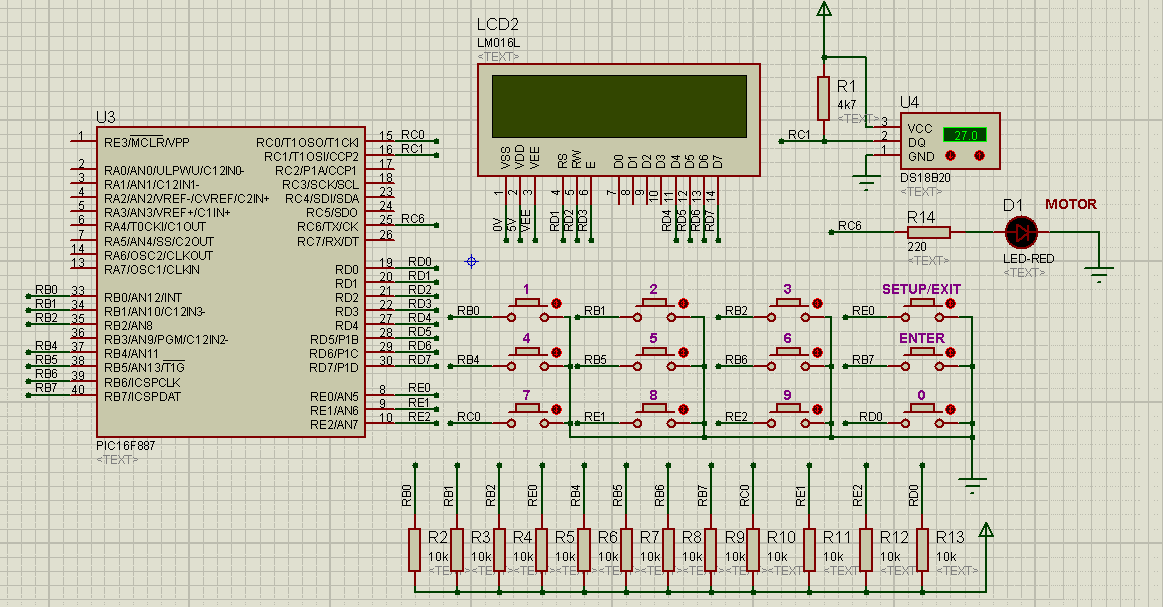
\includegraphics[scale=.5]{MACH_CHINH}
\end{center}
\caption{Mạch mô phỏng của đề tài với Protues}
\end{figure}
\newpage
\section{Kết quả làm mạch thực tế}
\begin{figure}[!h]
\begin{center}
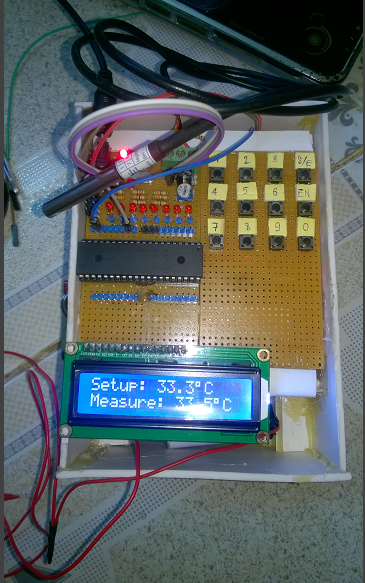
\includegraphics[width=.35\linewidth]{THUC-TE1}
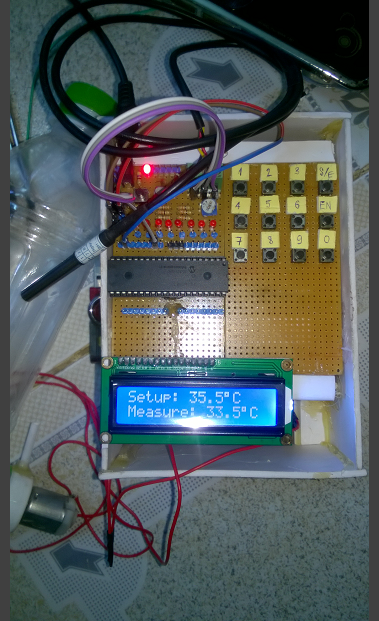
\includegraphics[width=.35\linewidth]{THUC-TE2}\\
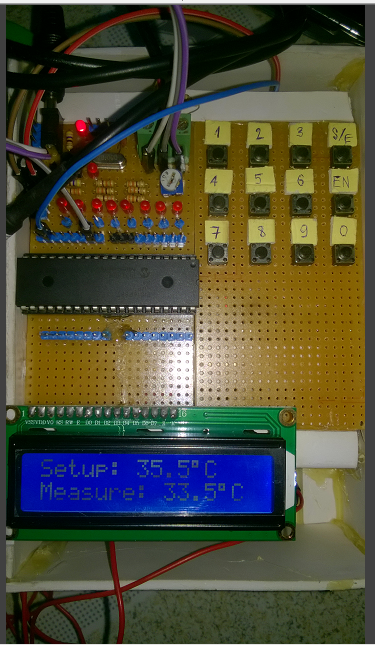
\includegraphics[width=.35\linewidth]{THUC-TE4}
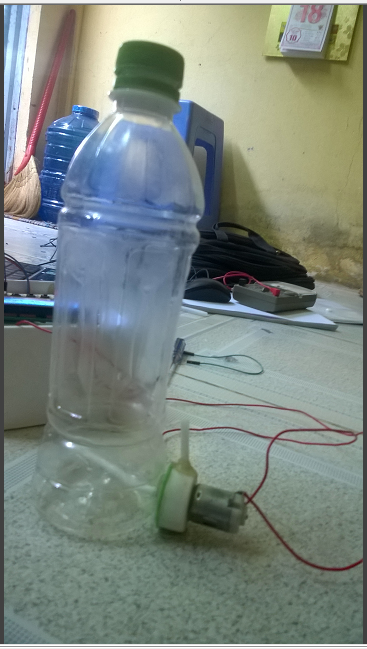
\includegraphics[width=.35\linewidth]{THUC-TE6}
\end{center}
\caption{Mạch làm thực tế của đề tài}
\end{figure}
\appendix
\part*{PHỤ LỤC}
\addcontentsline{toc}{part}{PHỤ LỤC}
\chapter{Các phần cứng và sơ đồ được dùng trong đề tài} \label{phancung-sodo}
\section*{Các phần cứng} \label{phuluc-phancung}
\begin{enumerate}
\item \textit{Vi điều khiển PIC 16F887}
\begin{figure}[h]
\begin{center}
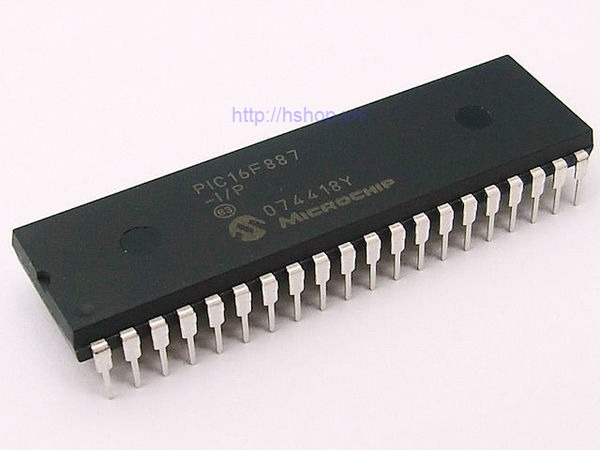
\includegraphics[scale=.3]{HW_16F887}
\end{center}
\caption{Vi điều khiển PIC 16F887}
\end{figure}

\item \textit{Cảm biến nhiệt độ DS18B20 (loại dây)}
\begin{figure}[h]
\begin{center}

\includegraphics[scale=.3]{HW_DS18B20} 
\end{center}
\caption{Cảm biến nhiệt độ DS18B20 (loại dây)} \label{DS18B200}
\end{figure}

\item \textit{Màn hình hiển thị LCD 1602}
\begin{figure}[h]
\begin{center}
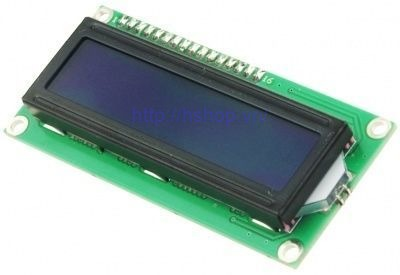
\includegraphics[scale=.35]{HW_LCD1602}
\end{center}
\caption{Màn hình hiển thị LCD 16x2} \label{LCD1602}
\end{figure}

\item \textit{Module 1 Relay với Opto cách ly kích H/L (5VDC)}
\begin{figure}[h]
\begin{center}
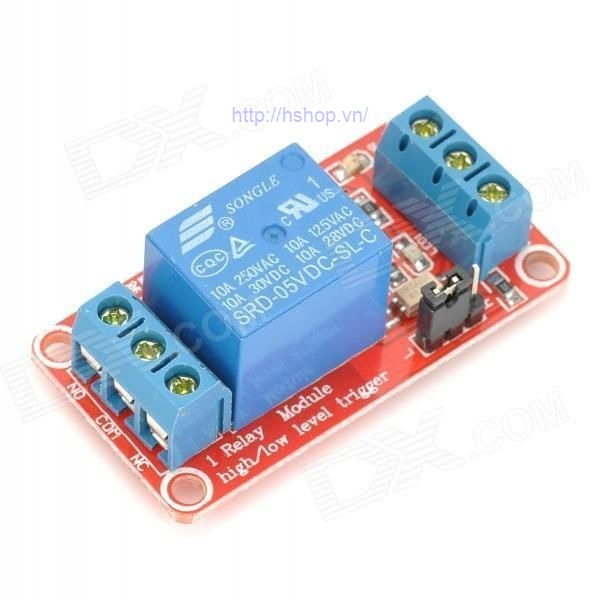
\includegraphics[scale=.2]{HW_RELAY}
\end{center}
\caption{Module Relay 5VDC với Opto cách ly}\label{RELAY}
\end{figure}

\item \textit{Mạch nạp cho vi điều khiển PIC}: mạch nạp hỗ trợ các dòng PIC: $10$, $12$, $12F$, $16C$, $16F$, $18F$.
\begin{figure}[h]
\begin{center}
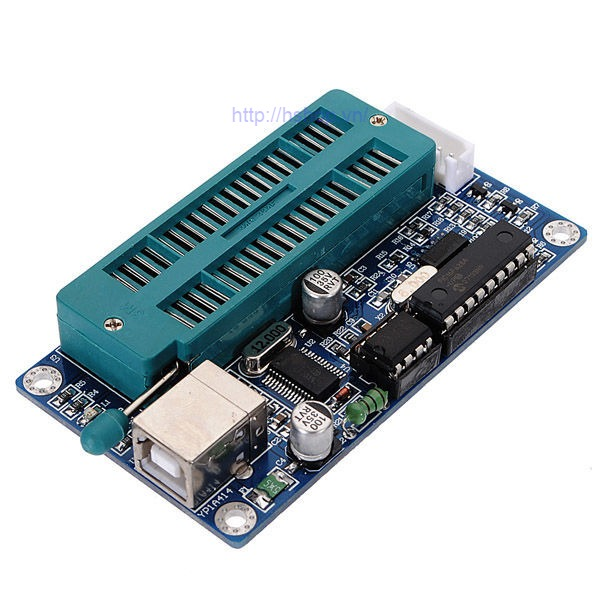
\includegraphics[scale=.25]{HW_PICKIT}
\end{center}
\caption{Mạch nạp PICKIT2 K150} 
\end{figure}
\newpage
\item \textit{Nút nhấn 4 chân}
\begin{figure}[h]
\begin{center}
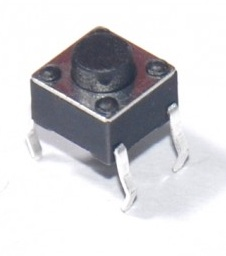
\includegraphics[scale=.3]{HW_BUTTON}
\end{center}
\caption{Nút nhấn loại 4 chân}
\end{figure}

\item \textit{Điện trở $4.7k\Omega$}
\begin{figure}[h]
\begin{center}
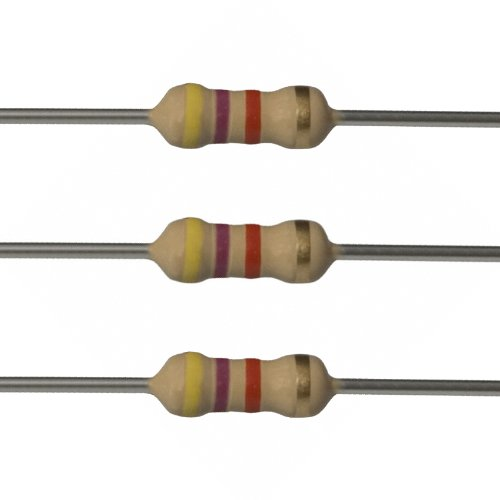
\includegraphics[scale=.2]{RES4k7}
\end{center}
\caption{Điện trở $4.7k\Omega$}
\end{figure}
\item \textit{Biến trở $10k\Omega$}
\begin{figure}[h]
\begin{center}
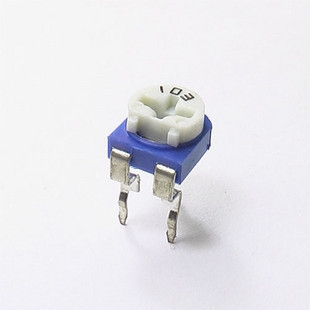
\includegraphics[scale=.3]{VAR_10k}
\end{center}
\caption{Biến trở $10k\Omega$}
\end{figure}
\newpage
\item \textit{Thạch anh tần số $20MHz$}
\begin{figure}[h]
\begin{center}
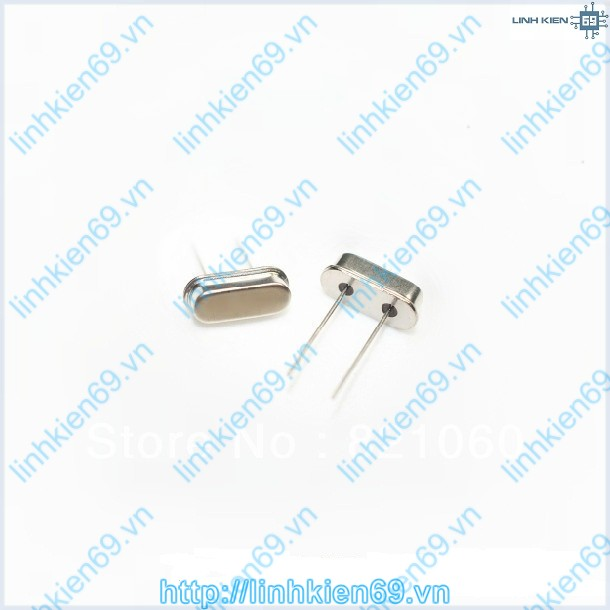
\includegraphics[scale=.15]{THACH_ANH}
\end{center}
\caption{Thạch anh tần số $20MHz$}
\end{figure}
\item \textit{Tụ điện $15pF$}
\begin{figure}[h]
\begin{center}
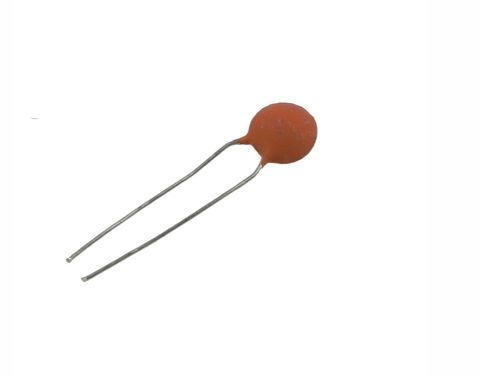
\includegraphics[scale=.5]{CAP}
\end{center}
\caption{Tụ điện $15pF$}
\end{figure}
\item \textit{Domino đấu nối loại 3 chân}
\begin{figure}[h]
\begin{center}
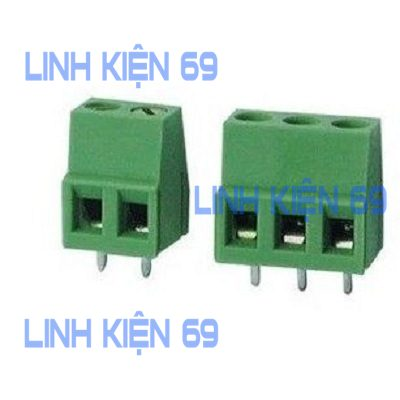
\includegraphics[scale=.4]{HW_DOMINO}
\end{center}
\caption{Domino đấu nối}
\end{figure}
\newpage
\item \textit{Đế IC 40 chân}
\begin{figure}[h]
\begin{center}
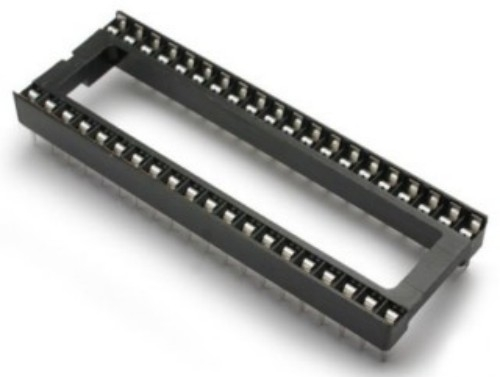
\includegraphics[scale=.3]{HW_DE_IC}
\end{center}
\caption{Đế IC 40 chân}
\end{figure}
\item \textit{Rào cái loại đơn}
\begin{figure}[h]
\begin{center}
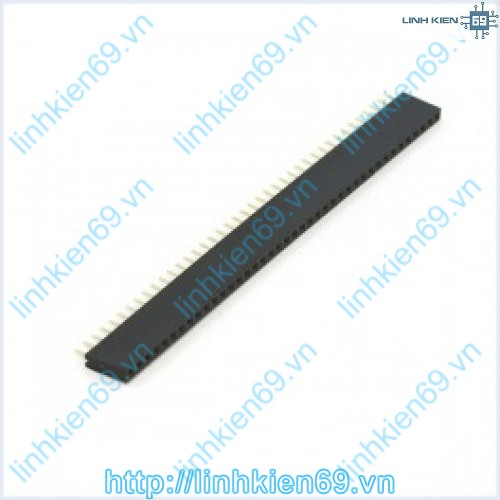
\includegraphics[scale=.25]{RAO_CAI}
\end{center}
\caption{Rào cái loại đơn}
\end{figure}
\item \textit{Rào đực loại đơn}
\begin{figure}[h]
\begin{center}
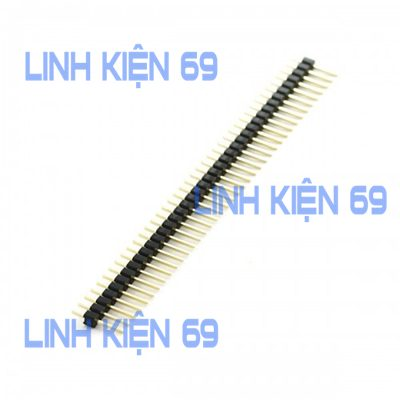
\includegraphics[scale=.35]{RAO_DUC}
\end{center}
\caption{Rào cái loại đơn}
\end{figure}
\newpage
\item \textit{Dây kết nối cái cái}
\begin{figure}[h]
\begin{center}
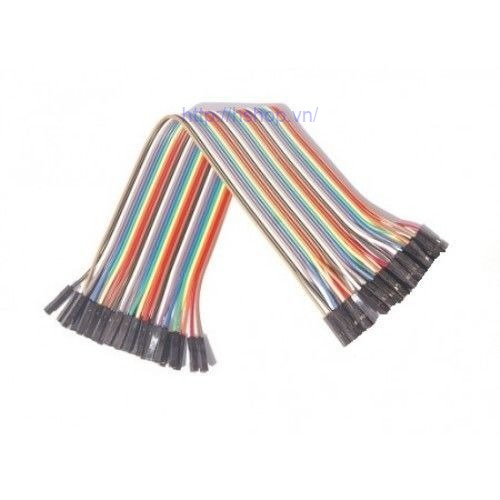
\includegraphics[scale=.3]{WIRE}
\end{center}
\caption{Dây kết nối 2 đầu cái - cái}
\end{figure}
\item \textit{Testboard hàn mạch}
\begin{figure}[h]
\begin{center}
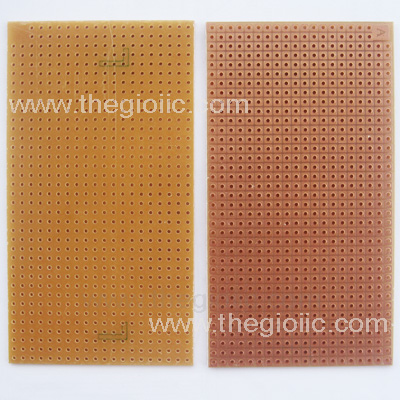
\includegraphics[scale=3]{TB_HAN}
\end{center}
\caption{Testboard hàn mạch}
\end{figure}
\item \textit{Động cơ 5VDC}
\begin{figure}[h]
\begin{center}
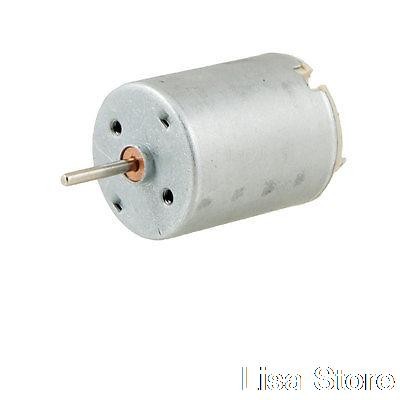
\includegraphics[scale=.3]{Motor}
\end{center}
\caption{Động cơ 5VDC}
\end{figure}
\item \textit{Bộ nguồn cấp cho vi điều khiển}: nguồn $5VDC - 2A$.
\item Các dụng cụ thực hành điện tử: VOM, mỏ hàn, chì hàn, kiềm, dây kết nối khi hàn, \ldots
\end{enumerate}
\chapter{Nội dung của các file thư viện được sử dụng trong chương trình}\label{lib}
\section{Định nghĩa PIC16F887 - file DEF\_887.H} \label{def887}
\begin{itemize}
\item Nguồn tham khảo: \textit{Tài liệu thực tập vi điều khiển} của thầy Đường Khánh Sơn. 
\item Nội dung của file \verb|DEF_887.H|:
\lstinputlisting[language=C]{DEF_887.H}
\end{itemize}
\section{Định nghĩa các chân được sử dụng trong đề tài - file DEF\_PIN.H} \label{defpin}
\begin{itemize}
\item Nội dung của file \verb|DEF_PIN.H|:
\lstinputlisting[language=C]{DEF_PIN.H}
\end{itemize}
\section{Thư viện LCD - file LCD\_LIB\_4BIT.C} \label{libLCD}
\begin{itemize}
\item Nguồn tham khảo: \textit{Tài liệu thực tập vi điều khiển} của thầy Đường Khánh Sơn. 
\item Nội dung:  sử dụng một số hàm truyền 4 bit dữ liệu.
\begin{itemize}
\item \verb|LCD_Init();| -- Khởi tạo LCD.
\item \verb|LCD_SetPosition(unsigned int cX);| -- Cài đặt vị trí con trỏ của LCD.
\item \verb|LCD_PutChar(unsigned int cX);| -- Viết ký tự hoặc chuỗi lên LCD.
\item \verb|LCD_PutCmd(unsigned int cX);| -- Gửi lệnh lên LCD.
\item \verb|LCD_PulseEnable();| -- Xung kích hoạt.
\item \verb|LCD_setData(unsigned int cX);| -- Đặt dữ liệu lên chân Data.
\end{itemize}
\item Nội dung của file \verb|LCD_LIB_4BIT.C|:
\lstinputlisting[language=C]{LCD_LIB_4BIT.C}
\end{itemize}
\section{Chuẩn giao tiếp một dây - file ONEWIRE.C} \label{ONEWIRE}
\begin{itemize}
\item Nguồn tham khảo: \verb|ytuonghay.vn|
\item Nội dung của file \verb|ONEWIRE.C|:
\lstinputlisting[language=C]{ONEWIRE.C}
\end{itemize}
\newpage
\section{Đọc nhiệt độ từ cảm biến DS18B20 - File DS18B20.C} \label{codeDS}
\begin{itemize}
\item Nguồn tham khảo: \verb|mcu.banlinhkien.vn|
\item Nội dung của file \verb|DS18B20.C|:
\lstinputlisting[language=C]{DS18B20.C}
\end{itemize}
\end{document}
